
\chapter{Disassembly of a sliding-stem control valve}

\label{valve_tour}

The following collection of photographs chronicles the complete disassembly of a Fisher E-body globe valve with pneumatic diaphragm actuator.  This control valve design is quite mature, but nevertheless enjoys wide application in modern industrial settings.  \index{Fisher E-body control valve}

\vskip 10pt

An important safety note when disassembling pneumatic control valves is to first relieve all tension from the actuator spring so that its stored energy cannot harm you or anyone else.  These springs may be quite large, exerting \textit{thousands of pounds} of force during normal operation.  

Spring tension may be relieved by moving the spring adjuster until it turns easily by hand without further aid of tools, or in the procedure shown in the following photographs by loosening the spanner nut attaching the actuator yoke to the valve bonnet.

\filbreak

This is the complete control valve, without a positioner attached.  What you see here is the actuator (painted green) and the valve body (painted grey), mounted on a steel plate for student learning in a laboratory setting.  The left-hand photograph shows the complete control valve assembly, while the right-hand photograph shows a student loosening the spanner nut holding the valve actuator yoke to the valve body:

$$\includegraphics[width=2.5in]{valve_teardown_01.eps} \hskip 30pt \includegraphics[width=2.5in]{valve_teardown_02.eps}$$

\filbreak

The next step is to un-couple the actuator stem from the valve stem.  On Fisher sliding-stem valves, this connection is made by a split block with threads matching those on each stem.  Removing two bolts from the block allows it to be taken apart (left-hand photograph).  Nuts threaded on to the valve stem, jammed up against the coupling block, must also be loosened before the stems may be uncoupled (right-hand photograph):

$$\includegraphics[width=2.5in]{valve_teardown_03.eps} \hskip 30pt \includegraphics[width=2.5in]{valve_teardown_04.eps}$$

It is very important that no spring tension exists on the stem prior to disassembly of the stem coupler, or else the two stems will slip past each other with great force once the coupler is removed.  Spring tension must be released, either by loosening the spring adjuster or by loosening the spanner nut holding the actuator yoke to the bonnet.

\filbreak

A close-up photograph of this stem connector block, with the front half removed for inspection, shows how it engages both threaded stems (valve and actuator) in a single nut-like assemblage.  The solid valve stem (below) slides into the hollow actuator stem (above), while the split connector ``nut'' engages the threads of both, holding the two stems together so they move up and down as one piece:

$$\includegraphics[width=4in]{valve_teardown_26.eps}$$

\filbreak

Once the actuator and valve body stems have been uncoupled, the actuator may be removed from the valve body entirely:

$$\includegraphics[width=4in]{valve_teardown_05.eps}$$

\filbreak

The bonnet is held to the rest of the valve body (in this case) by four large studs.  Removing the nuts on these studs allows the bonnet to be lifted off the body, exposing the valve trim for view:

$$\includegraphics[width=2.5in]{valve_teardown_06.eps} \hskip 30pt \includegraphics[width=2.5in]{valve_teardown_07.eps}$$

\filbreak

Seats in Fisher E-body globe valves rest in the bottom of the body, held in place by the cage surrounding the valve plug.  Once the bonnet is removed from the body, the seat may be removed without need of any specialized tools (left-hand photograph).  A view inside the body shows the place where the seat normally rests (right-hand photograph):

$$\includegraphics[width=2.5in]{valve_teardown_08.eps} \hskip 30pt \includegraphics[width=2.5in]{valve_teardown_09.eps}$$

\filbreak

With the bonnet removed, the plug and cage may be easily removed for inspection:

$$\includegraphics[width=4in]{valve_teardown_10.eps}$$

\filbreak

The packing follower (between the student's fingers) has been removed from the valve bonnet, and you can see the upper Teflon packing rings within the bonnet.  The student is also holding the packing flange in the same hand as the packing follower (left-hand photograph).  In the right-hand photograph, we see the student using a screwdriver to gently push the Teflon packing rings out of the bonnet, from the bottom side.  Care should be taken not to gouge or otherwise damage these rings during removal:

$$\includegraphics[width=2.5in]{valve_teardown_11.eps} \hskip 30pt \includegraphics[width=2.5in]{valve_teardown_12.eps}$$

\filbreak

The left-hand photograph shows all the packing components stacked on top of each other on the concrete floor, next to the bonnet.  From top to bottom you see the following components: a felt wiper, the packing follower, five (5) Teflon packing rings, a coil spring, and the packing box ring.  The right-hand photograph shows the same packing components stacked on the valve stem:

$$\includegraphics[width=2.5in]{valve_teardown_13.eps} \hskip 30pt \includegraphics[width=2.5in]{valve_teardown_14.eps}$$

\filbreak

Turning to the actuator, we begin disassembly by loosening the diaphragm hold-down bolts (left-hand photograph) and removing the upper half of the diaphragm casing (right-hand photograph).  A single bolt secures the upper diaphragm plate to the top of the actuator stem: 

$$\includegraphics[width=2.5in]{valve_teardown_15.eps} \hskip 30pt \includegraphics[width=2.5in]{valve_teardown_16.eps}$$

\filbreak

In the left-hand photograph you see the student removing the spring seat, having previously loosened the spring adjustor nut.  With the spring seat removed, the spring may be removed from the actuator assembly.  In the right-hand photograph the spring adjustor and spring seat have been removed from the actuator stem.  The student is now pointing at the valve spring, partially removed:

$$\includegraphics[width=2.5in]{valve_teardown_17.eps} \hskip 30pt \includegraphics[width=2.5in]{valve_teardown_18.eps}$$

\filbreak

Sliding the actuator diaphragm, plate, and stem out of the actuator assembly from the top of the actuator makes it easy to remove the large actuator spring (left-hand photograph).  The right-hand photograph shows all the moving actuator components re-assembled in their proper order outside of the yoke:

$$\includegraphics[width=2.5in]{valve_teardown_19.eps} \hskip 30pt \includegraphics[width=2.5in]{valve_teardown_20.eps}$$

\filbreak

The left-hand photograph shows the lower half of the actuator casing, with the student removing six (6) hold-down bolts joining this casing half to the actuator yoke.  The right-hand photograph shows the actuator casing half completely removed from the yoke, revealing a gasket and the bronze stem bushing (which serves to both guide the actuator stem and seal air pressure, since this is a reverse-acting actuator):

$$\includegraphics[width=2.5in]{valve_teardown_21.eps} \hskip 30pt \includegraphics[width=2.5in]{valve_teardown_22.eps}$$

\filbreak

A circular spring clip holds the stem bushing in the yoke casting.  The left-hand photograph shows the student using pliers to squeeze this spring clip and remove it from its groove cut into the metal of the yoke.  In the right-hand photograph, we see the student using the wooden handle of a hammer to gently tap the bushing out of the yoke.  The bushing has rubber O-ring seals between it and the yoke casting, so a small amount of force will be necessary to dislodge it.  Using the hammer's wooden handle to drive the bushing instead of a metal tool protects the relatively soft bronze bushing from impact damage.  Note how the student's right hand is waiting to catch the bronze bushing when it emerges from the hole, to protect it from falling against the hard concrete floor:

$$\includegraphics[width=2.5in]{valve_teardown_23.eps} \hskip 30pt \includegraphics[width=2.5in]{valve_teardown_24.eps}$$

\filbreak

The final photograph shows the bushing removed from its hole:

$$\includegraphics[width=4in]{valve_teardown_25.eps}$$












%%%%%%%%%%%%%%%%%%%%%%%%%%%%%%%%%%%%%%%%%%%%%%%%%%%%

